% Basic stuff
\documentclass[a4paper,10pt]{article}
\usepackage[utf8]{inputenc}
\usepackage[nswissgerman]{babel}
\usepackage{parskip}
\usepackage{ragged2e}

\usepackage{lipsum}

% 3 column landscape layout with fewer margins
\usepackage[landscape, left=0.75cm, top=1cm, right=0.75cm, bottom=1.5cm, footskip=15pt]{geometry}
\usepackage{flowfram}
\ffvadjustfalse
\setlength{\columnsep}{1cm}
\Ncolumn{4}

% define nice looking boxes
\usepackage[most]{tcolorbox}

% a base set, that is then customised
\tcbset {
  base/.style={
    boxrule=0mm,
    leftrule=1mm,
    left=1.75mm,
    arc=0mm,
    halign=left,
    fonttitle=\bfseries, 
    colbacktitle=black!10!white, 
    coltitle=black, 
    toptitle=0.75mm, 
    bottomtitle=0.25mm,
    title={#1},
  }
}

\definecolor{analysis-i}{RGB}{37, 170, 245}
\newtcolorbox{mainbox}[1]{
  colframe=analysis-i, 
  base={#1}
}

\newtcolorbox{subbox}[1]{
  colframe=black!20!white,
  base={#1}
}

% Mathematical typesetting & symbols
\usepackage{amsthm, mathtools, amssymb} 
\usepackage{marvosym, wasysym}
\allowdisplaybreaks

% Tables
\usepackage{tabularx, multirow}
\usepackage{booktabs}
\renewcommand*{\arraystretch}{2}

% Make enumerations more compact
\usepackage{enumitem}
\setitemize{itemsep=0.5pt}
\setenumerate{itemsep=0.75pt}

% To include sketches & PDFs
\usepackage{graphicx}

% For hyperlinks
\usepackage{hyperref}
\hypersetup{
  colorlinks=true
}

% Metadata
\title{Analysis I}
\author{Julian Steinmann}
\date{Sommersession 2021}

% Math helper stuff
\def\limn{\lim_{n\to \infty}}
\def\limxo{\lim_{x\to 0}}
\def\limxi{\lim_{x\to\infty}}
\def\limxn{\lim_{x\to-\infty}}
\def\sumk{\sum_{k=1}^\infty}
\def\sumn{\sum_{n=0}^\infty}
\def\N{\mathbb{N}}
\def\Z{\mathbb{Z}}
\def\R{\mathbb{R}}
\def\C{\mathbb{C}}
\def\dx{\text{ d}x}
\DeclareMathOperator{\arccot}{arccot}

\begin{document}

\maketitle

% Not actually an abstract. We abuse it for licencing
\renewcommand{\abstractname}{Lizenz}
\begin{abstract}
 Dieses Dokument ist unter CC BY-SA 3.0 lizenziert. Es darf verbreitet oder verändert werden, solange der Urheber und die Lizenz erhalten bleibt. \\

 \begin{center}
 Der \LaTeX-Quelltext ist verfügbar auf \\ \href{https://github.com/XYQuadrat/eth-cheatsheets}{github.com/XYQuadrat/eth-cheatsheets}.
 \end{center}
\end{abstract}

\RaggedRight

\section{Folgen}
\subsection{Konvergenz}
Eine Folge $(a_n)_{n\in \mathbb{N}}$ konvergiert gegen L \\ $\iff \lim_{n \to \infty} a_n = L $ \\ $\iff \forall \epsilon > 0 \ \exists N_e \ \forall n \ge N_\epsilon : \ | a_n - L | < e$\\

$\epsilon$ ist durch Konstante $C \in \R$ beschränkt.
Es gilt ausserdem:
\begin{itemize}
 \item konvergent $\implies$ beschränkt
 \item $(a_n)$ konvergent $\iff (a_n)$ beschränkt \textbf{und} \\$\lim \inf a_n = \lim \sup a_n$
\end{itemize}


\begin{subbox}{Limes superior/inferior}
\[ \limn \inf a_n := \limn \left( \inf \left\{ a_k : \: k \geq n \right\} \right) \]
\[ \limn \sup a_n := \limn \left( \sup \left\{ a_k : \: k \geq n \right\} \right) \]
\end{subbox}

\begin{subbox}{Sandwichsatz}
Wenn $\limn a_n = \alpha$, $\limn b_n = \alpha$ und $a_n \le c_n \le b_n \; \forall n \ge k$, dann $\limn c_n = \alpha$.
\end{subbox}

\begin{mainbox}{Weierstrass}
\begin{subbox}{}
$(a_n)_{n \geq 1}$ ist \emph{monoton wachsend} falls $a_n \leq a_{n+1} \; \forall n \geq 1$

$(a_n)_{n \geq 1}$ ist \emph{monoton fallend} falls $a_{n+1} \leq a_n \; \forall n \geq 1$
\end{subbox}
$a_n$ monoton wachsend und nach oben beschränkt $\implies$ $(a_n)_{n \geq 1}$ konvergiert ($\limn a_n = \sup \left\{ a_n : \ n \ge 1 \right\}$).

$a_n$ monoton fallend und nach unten beschränkt $\implies$ $(a_n)_{n \geq 1}$ konvergiert ($\limn a_n = \inf \left\{ a_n : \ n \ge 1 \right\}$).
\end{mainbox}

\begin{mainbox}{Cauchy-Kriterium}
Die Folge $(a_n)_{n \geq 1}$ ist genau dann konvergent, falls $\forall e > 0 \ \exists N \ge 1$ so dass $| a_n - a_m | < \epsilon \quad \forall n,m \ge N$.
\end{mainbox}

\subsubsection{Teilfolge}
Eine \emph{Teilfolge} von $(a_n)_{n \geq 1}$ ist eine Folge $(b_n)_{n \geq 1}$ wobei $b_n = a_{l(n)}$ und $l: \: \N^* \to \N^*$ eine Abbildung mit $l(n) < l(n+1) \quad \forall n \ge 1$ (z.B. $l(n) = 2n$). 

\subsubsection{Bolzano-Weierstrass}
\begin{mainbox}{}
Jede beschränkte Folge besitzt eine konvergente Teilfolge.
\end{mainbox}

\subsection{Strategie - Konvergenz von Folgen}
\begin{enumerate}
 \item Brüche: Grösste Potenz von $n$ kürzen, alle Brüche der Form $\frac{a}{n^a}$ streichen
 \item Wurzeln in Summe im Nenner: Zähler und Nenner mit der Differenz der Summe im Nenner multiplizieren (z.B. $(a+b)$ mit $(a-b)$).
 \item Rekursive Folgen: Weierstrass
 \item Sandwichsatz
 \item Mit bekannter Folge vergleichen.
 \item Grenzwert durch einfaches Umformen ermitteln
 \item Grenzwert per Definition der Konvergenz zeigen
 \item Cauchy-Kriterium
 \item Konvergenten Majoranten suchen
\end{enumerate}

\subsection{Strategie - Divergenz von Folgen}
\begin{enumerate}
 \item Suchen einer divergenten Vergleichsfolge
 \item Alternierende Folgen: Zeige, dass $\limn a_{l_1(n)} \ne \limn a_{l_2(n)}$
\end{enumerate}

\subsection{Tricks für Grenzwerte}
\subsubsection{Binome}
\begin{multline*}
    \lim_{x\to\infty} (\sqrt{x + 4} - \sqrt{x - 2}) \\
    = \lim_{x\to\infty} \frac{(x+4)-(x-2)}{\sqrt{x+4}+\sqrt{x-2}}
\end{multline*}

\subsubsection{Substitution}
$$\lim_{x\to\infty} x^2 (1-\cos(\frac{1}{x}))$$
Substituiere nun $u = \frac{1}{x}$:
\begin{multline*}
    \lim_{u \to 0} \frac{1 - \cos(u)}{u^2} \\
    = \lim_{u \to 0} \frac{\sin(u)}{2u} = \lim_{u\to 0} \frac{\cos(u)}{2} = \frac{1}{2}
\end{multline*}

\subsubsection{Induktive Folgen (Induktionstrick)}
\begin{enumerate}
  \item Geschlossene Form finden. Ansonsten:
  \item Zeige monoton wachsend / fallend
  \item Zeige beschränkt
  \item Weierstrass: Folge muss gegen einen Grenzwert konvergieren
  \item Verwende Induktionstrick:
  \begin{subbox}{Induktionstrick}
    $\limn{d_n} = d$ $\implies$ für jede Teilfolge $l(n)$ gilt $\limn{d_{l(n)}} = d$. Wähle also Teilfolge $l(n) := n + 1$, dann gilt $\limn{d_{n+1}} = d$.
  \end{subbox}
\end{enumerate}

\section{Reihen}

\begin{mainbox}{Cauchy-Kriterium für Reihen}
Die Reihe $\sumk a_k$ ist genau dann konvergent, falls $\forall \epsilon > 0 \ \exists N \ge 1$ mit $| \sum_{k=n}^m a_k | < \epsilon \ \forall m \ge n \ge N$.
\end{mainbox}

\subsubsection{Reihenarithmetik}
Wenn $\sumk a_k$ und $\sumk b_k$ konvergent sind, dann gilt:
\begin{itemize}
 \item $\sumk (a_k + b_k)$ konvergent und $\sumk (a_k + b_k) = \left( \sumk a_k \right) + \left( \sumk b_k \right)$
 \item $\sumk \alpha \cdot a_k$ konvergent und $\sumk \alpha \cdot a_k = \alpha \cdot \sumk a_k$
\end{itemize}

% % Soweit ich sehe das gleiche wie Majoranten-/Minorantenkriterium unten
% \begin{mainbox}{Vergleichssatz}
% Seien $\sumk a_k$ und $\sumk b_k$ Reihen mit $0 \le a_k \le b_k \forall k \ge K \ge 1$.
% $$\sumk b_k \text{ konv.} \implies \sumk a_k \text{ konv.}$$ 
% $$\sumk a_k \text{ div.} \implies \sumk b_k \text{ div.}$$
% \end{mainbox}

\begin{mainbox}{Nullfolgenkriterium}
\[ \limn \left| a_n \right| \neq 0 \implies \sumn{a_n} \text{ divergiert} \]
\end{mainbox}
Sanity-Check: Ist Folge $a_n$ in der Reihe keine Nullfolge, muss Reihe divergieren. Wegen Absolutbetrag lassen sich $(-1)^n$-Terme gut eliminieren.

\begin{mainbox}{Majorantenkriterium}
Sei $\left| a_n \right| \leq b_n \; \forall n \geq n_0, n_0 \in \N$.
\[ \sumn{b_n} \text{ konv.} \implies \sumn{a_n} \text{ konv. abs.} \]
\end{mainbox}
Vorgehen: Suche Folge $b_n$ mit $\left| a_n \right| \leq b_n$, deren Reihe konvergiert.

\begin{mainbox}{Minorantenkriterium}
Sei $0 \leq b_n \leq a_n \; \forall n \geq n_0, n_0 \in \N$
\[ \sumn{b_n} \text{ div.} \implies \sumn{a_n} \text{ div.} \]
\end{mainbox}
Vorgehen: Suche Folge $0 \leq b_n \leq a_n$, deren Reihe divergiert.

Als Majorant / Minorant oft geeignet:
\subsubsection{Geometrische Reihe} 
$\sum_{k=0}^\infty q^n$ konv. für $|q| < 1$ bzw. div. für $|q| \ge 1$
\subsubsection{Zeta-Funktion}
$\zeta(s) = \sum_{n=1}^\infty \frac{1}{n^s}$ konv. für $s > 1$ bzw. div. für $s \le 1$.
\emph{Harmonische Reihe} ist Spezialfall: $\zeta(1)$.

\begin{mainbox}{Leibnizkriterium}
Sei $(a_n)_{n \in \N}$.
\renewcommand{\labelenumi}{(\roman{enumi})}
\begin{enumerate}
    \item $a_n \xrightarrow{n \to \infty} 0$
    \item $a_n$ wird monoton (ab einem gewissen $n_0$)
\end{enumerate}
(i), (ii) $\implies$ $\sumn{(-1)^n a_n}$ konvergiert
\end{mainbox}
Wenn mit Majorantenkriterium zu grob abgeschätzt wurde, also Harmonische Reihe $\sum_{n=1}^\infty \frac{1}{n}$ divergiert, aber alternierende Harmonische Reihe $\sum_{n=1}^\infty \frac{(-1)^n}{n}$ konvergiert, kann Leibniz helfen.

\begin{mainbox}{Quotienten-/Wurzelkriterium}
\begin{itemize}
    \item \textbf{Quotientenkriterium:} \[ \limn{\left| \frac{a_{n+1}}{a_n} \right|} = q \]
    \item \textbf{Wurzelkriterium:} \[ \limn{\sqrt[n]{\left| a_n \right|}} = q \]
\end{itemize}
Mit \(
\begin{cases}
    q < 1 &\implies \sum_{n=1}^\infty \text{ konv. abs.} \\
    q = 1 &\implies \text{ keine Aussage} \\
    q > 1 &\implies \sum_{n=1}^\infty \text{ div.}
\end{cases}
\)
\end{mainbox}

% https://de.wikipedia.org/w/index.php?title=Integralkriterium&curid=303520
\begin{subbox}{Integralkriterium}
Sei $p \in \Z, \, f: \: \left[ p, \infty \right[ \to \left[ 0, \infty \right[$ monoton fallend.
\begin{multline*}
    f \text{ auf } \left[p, \infty \right[ \text{ integrierbar} \\
    \iff \sum_{n=p}^\infty f(n) \text{ ist konvergent}
\end{multline*}
\end{subbox}

\subsection{Absolute Konvergenz}
$\sumk a_k$ heisst \emph{absolut konvergent}, wenn $\sumk |a_k|$ konvergiert. 

Anwendung des Cauchy-Kriteriums: Eine absolut konvergente Reihe ist immer auch konvergent, es gilt $|\sumk a_k| \le \sumk |a_k|$.

Falls eine Reihe absolut konvergiert, konvergiert jede Umordnung der Reihe mit dem selben Grenzwert.

Falls die Reihe hingegen nur konvergiert, so gibt es immer eine Anordnung, so dass $\sum_{k=1}^\infty a_{\phi(k)} = x, \ \forall x\in \R$.

\subsection{Cauchy-Produkt}
\begin{subbox}{Cauchy-Produkt}
  Das Cauchy-Produkt von zwei Reihen $\sum_{i = 0}^\infty a_i$ und $\sum_{j = 0}^\infty b_j$ ist die Reihe
  \begin{multline*}
      \sum_{n=0}^\infty \left( \sum_{j=0}^n a_{n-j} b_j \right) \\
      = a_0b_0 + (a_0b_1 + a_1b_0) + \ldots
  \end{multline*}
  Es konvergiert, falls beide Reihen konvergieren.
\end{subbox}

\subsection{Wichtige Reihen}
\begin{align*}
 \sum_{i=1}^n i &= \frac{n(n+1)}{2} \\
 \sum_{i=1}^n i^2 &= \frac{1}{6}n(n+1)(2n+1) \\
 \sum_{i=1}^n i^3 &= \frac{1}{4}n^2(n+1)^2 \\
 \sum_{i=1}^\infty \frac{1}{i^2} &= \frac{\pi^2}{6} \\
 \sum_{n=1}^\infty \frac{1}{n(n+1)} &= 1
\end{align*}

\subsection{Strategie - Konvergenz von Reihen}
% \begin{enumerate}
% %  \item Ist Reihe ein bekannter Typ? (Teleskopieren, Geometrische/Harmonische Reihe, Zetafunktion, ...)
% %  \item Ist $\limn a_n = 0$? Wenn nein, divergent.
% %  \item Quotientenkriterium \& Wurzelkriterium anwenden
% %  \item Vergleichssatz anwenden, Vergleichsreihen suchen
% %  \item Leibnizkriterium anwenden
% %  \item Integral-Test anwenden (Reihe zu Integral)
% \end{enumerate}
\begin{enumerate}
    \item Bekannter Reihentyp?
    \item Nullfolgenkriterium
    \item (Weierstrass für Reihen)
    \item (Cauchy für Reihen)
    \item Vergleich mit Referenzreihen (Min.-/Maj.- Kriterien)
    \item (Kompatibilität mit Add./Mult.)
    \item Leibnizkriterium
    \item Quotientenkriterium
    \item Wurzelkriterium
    \item Teleskopsummen
    \item Integralkriterium
\end{enumerate}
Beachte Unterschied zwischen \emph{absoluter Konvergenz} und "normaler" \emph{Konvergenz}!

\section{Funktionen}
\subsection{Stetigkeit}
Sei $f : D \to \R^d, x \to f(x)$ eine Funktion in $D \subseteq \R^d$.
\begin{mainbox}{Stetigkeit}
 $f$ ist \emph{in $x_0 \in D$ stetig}, falls es $\forall \epsilon > 0 \, \exists \delta > 0$, so dass $\forall x \in D$ gilt:
 \[ \left| x - x_0 \right| < \delta \implies \left| f(x) - f(x_0) \right| < \epsilon \]
 
 $f$ ist \emph{stetig}, falls sie in jedem Punkt von $D$ stetig ist.
\end{mainbox}
Polynomiale Funktionen sind auf $\R$ stetig.
\begin{subbox}{}
 Falls $f$ und $g$ den gleichen Definitions-/Bildbereich haben und in $x_0$ stetig sind, dann sind auch $f + g$, $\lambda \cdot f$, $f \cdot g$, $\frac{f}{g}$, $|f|$, $\max(f,g)$, $\min(f,g)$ stetig in $x_0$.
\end{subbox}


\begin{mainbox}{Zwischenwertsatz}
 Sei $I \in \R$, $f: \: I \to \R$ stetig und $a, b \in I$. Für jedes $c$ ($f(a) \leq c \leq f(b)$) gibt es ein $z$ ($a \leq z \leq b$) mit $f(z) = c$.
 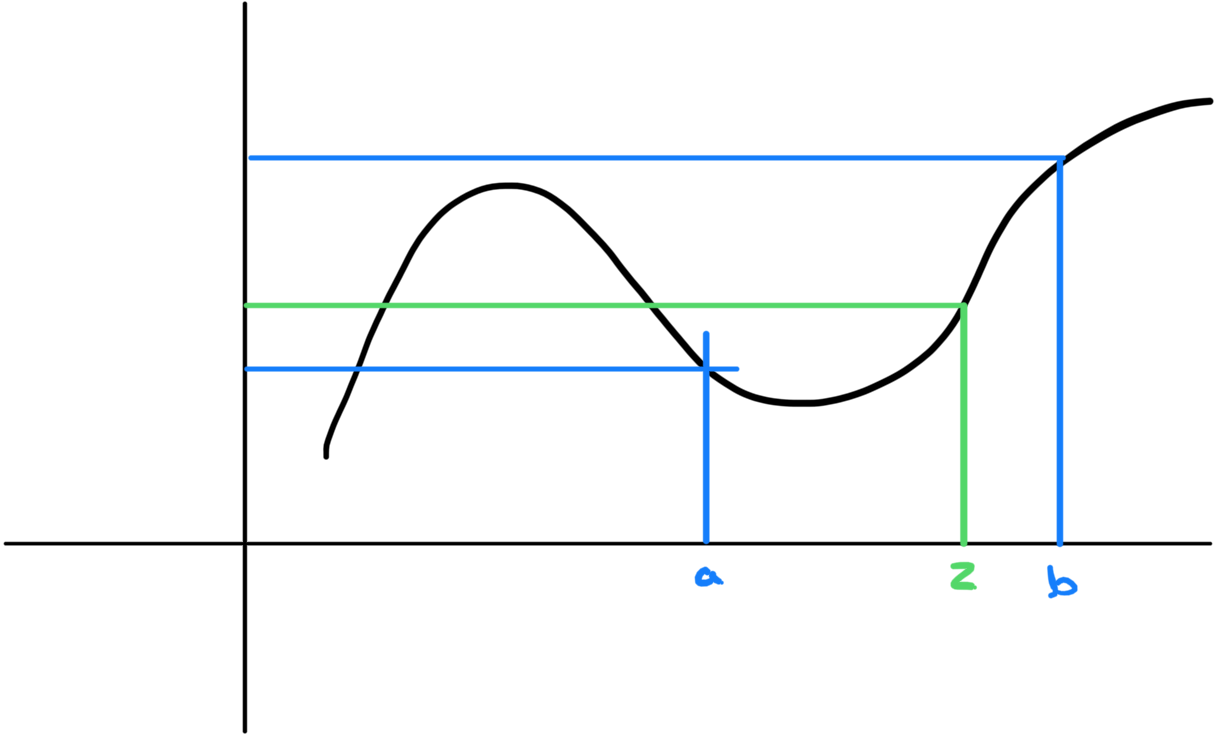
\includegraphics[width=\linewidth]{Zwischenwertsatz.png}
\end{mainbox}
Wird häufig verwendet um zu zeigen, dass eine Funktion einen gewissen Wert (z.B. Nullstelle) annimmt.

Daraus folgt, dass ein Polynom mit ungeradem Grad mindestens eine Nullstelle in $\R$ besitzt.

\subsubsection{Kompaktes Intervall}
Ein Intervall $I \in \R$ ist kompakt, falls es von der Form $I = [a,b]$ mit $a \le b$ ist.

\begin{subbox}{}
Sei $(x_n)_{n \geq 1}$ konvergent mit $\limn{x_n} \in \R$. Sei $a \leq b$. Falls $\left\{ x_n: \: n \geq 1 \right\} \subseteq \left[ a, b \right]$, folgt $\limn{x_n} \in \left[ a, b \right]$.
\end{subbox}

\begin{mainbox}{Min-Max-Satz}
 Sei $f: I = [a,b] \to \R$ stetig auf kompaktem Intervall $I$. Dann gibt es $u, v \in I$ mit $f(u) \le f(x) \le f(v) \; \forall x \in I$. Insbesondere ist $f$ beschränkt.
\end{mainbox}

\begin{subbox}{Stetigkeit unter Verknüpfung}
 Sei $D_1, D_2 \subseteq \R$, $f: \: D_1 \to D_2, \, g: D_2 \to \R$ und $x_0 \in D_1$. Falls $f$ in $x_0$ und $g$ in $f(x_0)$ stetig sind, ist $g \circ f: \: D_1 \to \R$ in $x_0$ stetig.
\end{subbox}

\begin{mainbox}{Satz über die Umkehrabbildung}
 Sei $f: I \to \R$ stetig und streng monoton. Dann ist $J := f(I) \subseteq \R$ ein Intervall und $f^{-1}: \: J \to I$ stetig und streng monoton.
\end{mainbox}

\begin{subbox}{Die reelle Exponentialfunktion}
 $\exp: \: \R \to \left] 0,+\infty \right[$ ist streng monoton wachsend, stetig und surjektiv.
 
 Dasselbe gilt auch für die Umkehrfunktion $\ln: \: \left] 0,+\infty \right[ \to \R$.
\end{subbox}

\subsection{Konvergenz von Funktionenfolgen}

\begin{mainbox}{Punktweise Konvergenz}
  $(f_n)_{n \geq 0}$ \emph{konvergiert punktweise} gegen $f: \: D \to \R$ falls $\limn f_n(x) = f(x)$ für alle $x \in D$ gilt.
\end{mainbox}

\begin{mainbox}{Gleichmässige Konvergenz}
 Die Folge $f_n : \: D \to \R$ \emph{konvergiert gleichmässig} in $D$ gegen $f: \: D \to \R$ falls gilt: $\forall \epsilon > 0 \ \exists N \ge 1$, so dass $\forall n \ge N, \ \forall x \in D: \: | f_n(x) - f(x) | < \epsilon$.
 
 Alternativ: $f_n: \: D \to \R$ ist \emph{gleichmässig konvergent}, falls $\limn f_n(x) = f(x)$ für alle $x\in D$ existiert und die Folge $(f_n)_{n \geq 0}$ gleichmässig gegen $f$ konvergiert.
\end{mainbox}
$\sum_{k=0}^\infty f_k(x)$ konvergiert gleichmässig, falls die durch $S_n(x) := \sum_{k=0}^n f_k(x)$ definierte Funktionenfolge gleichmässig konvergiert.

\begin{subbox}{}
 Sei $f_n: \: D \to \R$ eine Folge stetiger Funktionen. Sei $|f_n(x)| \le c_n \; \forall x \in D$ und $\sum_{n=0}^\infty c_n$ konvergiert. Dann konvergiert die Reihe $\sum_{n=0}^\infty f_n(x)$ gleichmässig und deren Grenzwert $f(x) := \sumn{f_n(x)}$ ist eine in $D$ stetige Funktion.
\end{subbox}

\subsection{Potenzreihen}
\begin{subbox}{Potenzreihe}
 Potenzreihen sind von der Form $\sum_{k=0}^\infty c_k x^k$. Eine Potenzreihe mit Entwicklungspunkt $x_0$ wird als $\sum_{n=0}^\infty a_n(x-x_0)^n$ definiert.
\end{subbox}

\begin{mainbox}{Konvergenzradius}
 Der Konvergenzradius $\rho$ einer Potenzreihe um einen Entwicklungspunkt $x_0$ ist die grösste Zahl $r$, so dass die Potenzreihe für alle $x$ mit $|x - x_0| < r$ konvergiert.
 
 Sei $l = \limsup_{k \to \infty} \sqrt[k]{|c_k|}$. Eine Potenzreihe hat \emph{positiven Konvergenzradius}, falls $l$ existiert. Dann gilt
 \[ \rho = \begin{cases}
     +\infty & \text{falls } l = 0 \\
     \frac{1}{l} & \text{falls } l > 0
 \end{cases} \]
\end{mainbox}
$\sum_{k=0}^\infty a_n x^n$ konvergiert absolut für alle $|x| < \rho$ und divergiert für alle $|x| > \rho$. Der Fall $|x| = \rho$ ist unklar und muss geprüft werden.
\subsubsection{Definitionen per Potenzreihen}
\begin{align*}
\exp(x) &= \sumn \frac{x^n}{n!} & \rho &= \infty \\
\sin(x) &= \sumn (-1)^n \frac{x^{2n + 1}}{(2n + 1)!} & \rho &= \infty \\
\cos(x) &= \sumn (-1)^n \frac{x^{2n}}{(2n)!} & \rho &= \infty \\
\ln(x + 1) &= \sumk (-1)^{k+1} \frac{x^k}{k} & \rho &= 1
\end{align*}

\subsection{Grenzwerte von Funktionen}
\begin{subbox}{Häufungspunkt}
 $x_0 \in \R$ ist ein \emph{Häufungspunkt} der Menge D falls $\forall \delta > 0$: $(]x_0 - \delta, x_0 + \delta[ \setminus \{x_0\}) \cap D \ne \varnothing$.
\end{subbox}

\begin{mainbox}{Grenzwert}
 Sei $f: \: D \to \R$, $x_0 \in \R$ ein Häufungspunkt von $D$. Dann ist $A \in \R$ der \emph{Grenzwert von $f(x)$ für $x \to x_0$} ($\lim_{x\to x_0} f(x) = A$), falls $\forall \epsilon > 0 \ \exists \delta > 0$, so dass $\forall x \in D \cap (]x_0 - \delta, x_0 + \delta[ \setminus \{x_0\}): |f(x) - A| < \epsilon$.
\end{mainbox}

\begin{subbox}{Satz von L'Hospital}
  Seien $f,g$ stetig und differenzierbar auf $]a,b[$. Wenn $\lim_{x\to c} f(x) = \lim_{x \to c} g(x) = 0$ oder $\pm \infty$ und $g'(x) \ne 0 \ \forall x \in I \backslash \{c\}$, dann gilt $$\lim_{x\to c} \frac{f(x)}{g(x)} = \lim_{x\to c}\frac{f'(x)}{g'(x)}$$
\end{subbox}

Grenzwerte der Form $\infty^0$ und $1^\infty$ können meist mit $f(x)^{g(x)} = e^{g(x)\cdot \ln(f(x))}$ und dann Bernoulli (nur Exponenten betrachten da $e$ stetig) anwenden oder vereinfachen berechnet werden.

\section{Ableitungen}
\subsection{Differenzierbarkeit}
\begin{mainbox}{Differenzierbar}
\begin{mainbox}{}
 $f$ ist \emph{in $x_0$ differenzierbar}, falls der Grenzwert $\lim_{x\to x_0} \frac{f(x) - f(x_0)}{x - x_0}$ existiert. Ist dies der Fall, wird der Grenzwert mit $f'(x_0)$ bezeichnet.
\end{mainbox}

Alternativ mit $x = x_0 + h$:
\begin{subbox}{}
\[ f'(x_0) = \lim_{h \to 0} \frac{f(x_0 + h) - f(x_0)}{h} \]
\end{subbox}

 $f$ ist \emph{differenzierbar}, falls $f$ für jedes $x_0 \in D$ differenzierbar ist.
\end{mainbox}
\begin{subbox}{Differenzierbarkeit nach Weierstrass}
Sei $f: \: D \to \R$, $x_0 \in D$ Häufungspunkt von $D$. Folgende Aussagen sind äquivalent:
\begin{enumerate}
    \item $f$ ist in $x_0$ differenzierbar.
    \item Es gibt $c \in \R$ und $r: \: D \to \R$ mit:
    \begin{enumerate}
        \item $f(x) = f(x_0) + c(x - x_0) + r(x)(x - x_0)$
        \item $r(x_0) = 0$ und $r$ ist stetig in $x_0$.
    \end{enumerate}
\end{enumerate}
Falls dies zutrifft ist $c = f'(x_0)$ eindeutig bestimmt.
\end{subbox}
Vereinfachung mit $\phi(x) = f'(x_0) + r(x)$:
$f$ ist genau dann in $x_0$ differenzierbar, falls es $\phi: \: D \to \R$ gibt, die stetig in $x_0$ ist und so, dass
\[ f(x) = f(x_0) + \phi(x)(x - x_0) \; \forall x \in D \text{.} \]
In diesem Fall gilt $\phi(x_0) = f'(x_0)$.

\begin{mainbox}{Höhere Ableitungen}
 \begin{enumerate}
  \item Für $n \ge 2$ ist $f$ \emph{n-mal differenzierbar in $D$} falls $f^{(n-1)}$ in $D$ differenzierbar ist. Dann ist $f^{(n)} := (f^{(n-1)})'$ die n-te Ableitung von $f$.
  \item $f$ ist \emph{n-mal stetig differenzierbar in $D$}, falls sie n-mal differenzierbar ist und $f^{(n)}$ in $D$ stetig ist.
  \item $f$ ist in $D$ \emph{glatt}, falls sie $\forall n \ge 1$ n-mal differenzierbar ist (''unendlich differenzierbar``).
 \end{enumerate}
\end{mainbox}
Glatte Funktionen: $\exp$, $\sin$, $\cos$, $\sinh$, $\cosh$, $\tanh$, $\ln$, $ \arcsin$, $\arccos$, $\arccot$, $\arctan$ und alle Polynome. $\tan$ ist auf $\R \setminus \{\frac{\pi}{2} + k\pi\}$, $\cot$ auf $\R \setminus \{k\pi\}$ glatt.

\subsection{Ableitungsregeln}

\begin{itemize}
  \item Linearität der Ableitung
  $$(\alpha \cdot f(x) + g(x))' = \alpha \cdot f'(x) + g'(x)$$
  \item Produktregel
  $$(f(x) \cdot g(x))' = f'(x) \cdot g(x) + f(x) \cdot g'(x)$$
  \item Quotientenregel
  $$\left(\frac{f(x)}{g(x)}\right)' = \frac{f'(x) \cdot g(x) - f(x) \cdot g'(x)}{g(x)^2}$$
  \item Kettenregel
  $$(f(g(x)))' = g'(x) \cdot f'(g(x))$$
  \item Potenzregel
  $$(c \cdot x^a)' = c \cdot a \cdot x^{a - 1}$$
\end{itemize}

\subsection{Implikationen der Ableitung}
\begin{itemize}
  \item $f$ besitzt ein \emph{lokales Maximum} in $x_0$, wenn $f'(x_0) = 0$ und $f''(x_0) < 0$ oder falls Vorzeichen von $f'$ um $x_0$ von $+$ zu $-$ wechselt.
  \item $f$ besitzt \emph{lokales Minimum} in $x_0$, wenn $f'(x_0) = 0$ und $f''(x_0) > 0$ oder falls Vorzeichen von $f'$ um $x_0$ von $-$ zu $+$ wechselt.
  \item $f$ besitzt \emph{lokales Extremum} in $x_0$, wenn $f'(x_0) = 0$ und $f''(x_0) \ne 0$.
  \item $f$ besitzt \emph{Sattelpunkt} in $x_0$, wenn $f'(x_0) = 0$ und $f''(x_0) = 0$.
  \item $f$ besitzt \emph{Wendepunkt} in $x_0$, wenn $f''(x_0) = 0$.
  \item $f$ ist in $x_0$ \emph{konvex}, wenn $f''(x_0) \ge 0$ (\emph{streng konvex} mit $>$).
  \item $f$ ist in $x_0$ \emph{konkav}, wenn $f''(x_0) \le 0$ (\emph{streng konkav} mit $<$).
\end{itemize}

\subsection{Sätze zur Ableitung}
\begin{subbox}{Satz von Rolle}
 Sei $f: [a,b] \to \R$ stetig und in $]a,b[$ differenzierbar. Wenn $f(a) = f(b)$, gibt es ein $\xi \in ]a,b[$ mit $f'(\xi) = 0$.
 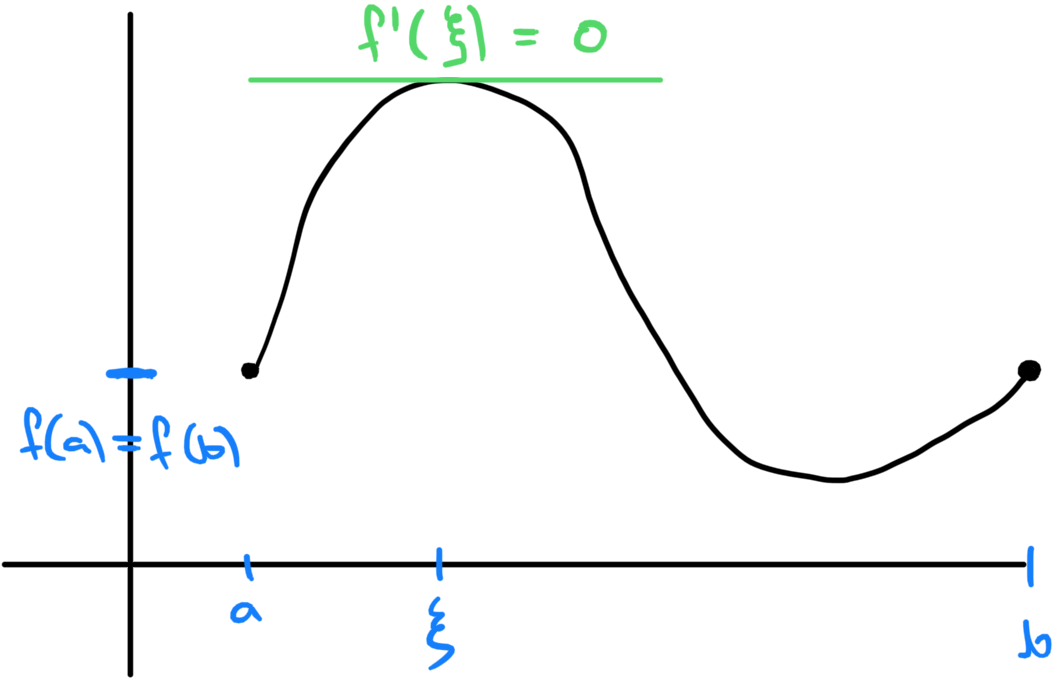
\includegraphics[width=\linewidth]{Satz von Rolle.png}
\end{subbox}
\begin{mainbox}{Mittelwertsatz (Lagrange)}
 Sei $f: [a,b] \to \R$ stetig und in $]a,b[$ differenzierbar. Dann gibt es $\xi \in ]a,b[$ mit $f(b) - f(a) = f'(\xi)(b-a)$.
 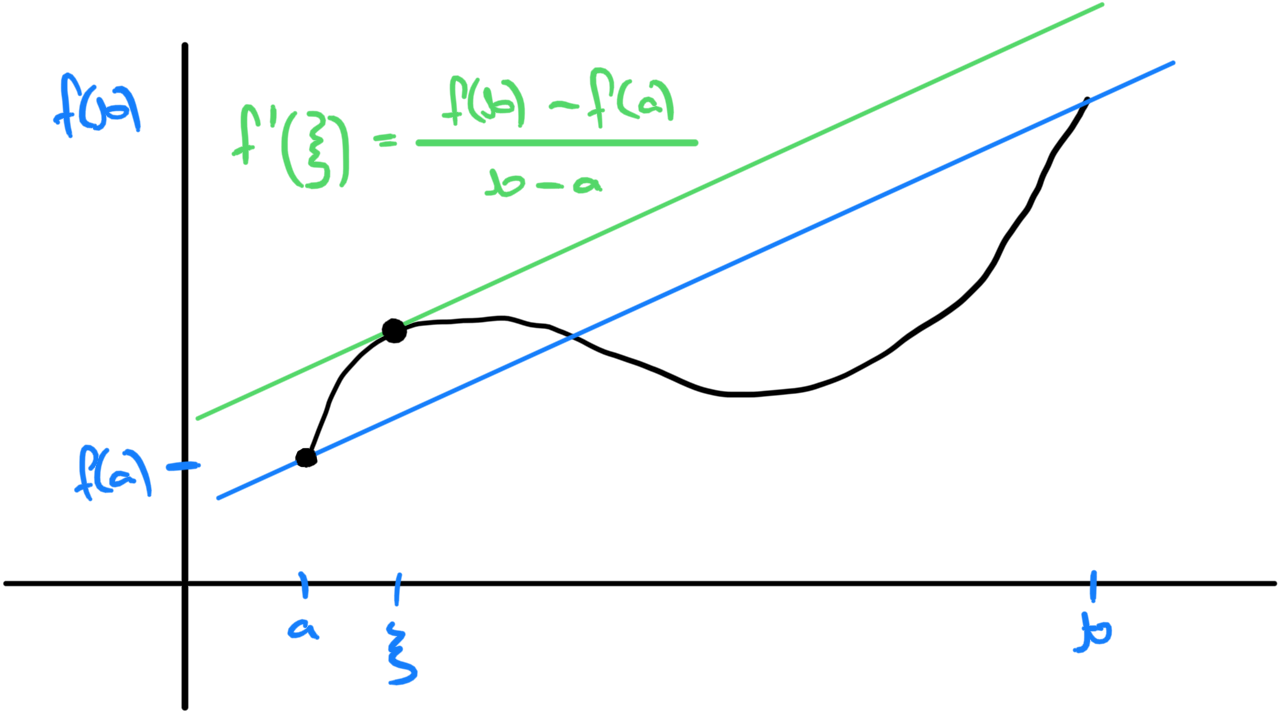
\includegraphics[width=\linewidth]{Lagrange.png}
\end{mainbox}

\subsection{Taylorreihen}
Jede glatte Funktion $f \in \C^\infty$ kann als Potenzreihe (Taylorreihe) angenähert werden.

\begin{subbox}{Taylor-Polynom}
 Das N-te Talyor-Polynom $T_N f(x; a)$ an einer Entwicklungsstelle $a$ ist definiert als:
 \begin{multline*}
    T_n f(x; a) := \sum_{n=0}^{N} \frac{f^{(n)} (a)}{n!} (x - a)^n \\
    = f(a) + f'(a) \cdot (x-a) \\
    + \frac{f''(a)}{2} \cdot (x - a)^2 + \ldots
 \end{multline*}
\end{subbox}

\begin{mainbox}{Taylorreihe}
 Taylorreihe von $f$ an Stelle $a$:
 \begin{multline*}
     Tf(x;a) := T_\infty \\
     = \sumn \frac{f^{(n)}(a)}{n!} \cdot (x-a)^n
 \end{multline*}
\end{mainbox}
Beispiele Taylorreihen ($a = 0$):
\begin{itemize}
 \item $\sin(x) = \sumn (-1)^n \cdot \frac{x^{2n+1}}{(2n+1)!}$
 \item $\cos(x) = \sumn (-1)^n \cdot \frac{x^{2n}}{(2n)!}$
 \item $e^x = \sumn \frac{x^n}{n!}$
 \item $e^{-x} = \sumn (-1)^n \cdot \frac{x^n}{n!}$
 \item $\sinh(x) = \sumn \frac{x^{2n+1}}{(2n+1)!}$
 \item $\cosh(x) = \sumn \frac{x^{2n}}{(2n)!}$
\end{itemize}

\section{Integrale}
\subsection{Riemann-Integral}
\begin{subbox}{Partition}
 Eine \emph{Partition} von $I$ ist eine endliche Teilmenge $P \subsetneq [a,b]$, wobei $\{a,b\} \subseteq P$.
\end{subbox}
\begin{subbox}{Unter- und Obersumme}
Wir bezeichnen mit $\delta_i := x_i - x_{i - 1}, \, i \geq 1$ die Länge des Teilintervalls $[x_{i - 1}, x_i$.

Untersumme:
\[ s(f, P) := \sum_{i=1}^n f_i \delta_i, \, f_i = \inf_{x_{i - 1} \leq x \leq x_i} f(x) \]

Obersumme:
\[ S(f, P) := \sum_{i=1}^n F_i \delta_i, \, F_i = \sup_{x_{i - 1} \leq x \leq x_i} f(x) \]
\end{subbox}
\begin{mainbox}{Riemann-Integrierbarkeit}
 $f:[a,b] \to \R$ ist \emph{Riemann-integrierbar} (kurz: \emph{integrierbar}), falls $s(f) = S(f)$. Dann ist $\int_a^b f(x) \, dx := s(f) = S(f)$.
\end{mainbox}
\begin{subbox}{Riemannsche Summe}
Sei $P = {x_0, \dots, x_n}$ eine Partition.
\[ \delta(P) := \max_{1 \leq i \leq n} (x_i - x_{i - 1}) \]
Zudem wählen wir für alle $1 \leq i \leq n$ $\xi_i \in [x_{i - 1}, x_i]$. Dann ist
\[ \sigma := \sum_{i=1}^n f(\xi_i)d_i \]
eine \emph{Riemannsche Summe}.
\end{subbox}

\subsection{Integrierbarkeit zeigen}
\begin{itemize}
 \item $f$ stetig in $[a,b] \implies f$ integrierbar über $[a,b]$
 \item $f$ monoton in $[a,b] \implies f$ integrierbar über $[a,b]$
 \item Wenn $f,g$ beschränkt und integrierbar sind, dann sind $f+g$, $\lambda \cdot f$, $f \cdot g$, $|f|$, $\max(f,g)$, $\min(f,g)$ und $\frac{f}{g}$ integrierbar.
 \item Jedes Polynom ist integrierbar, auch $\frac{P(x)}{Q(x)}$ falls $Q(x)$ in $[a,b]$ keine Nullstellen besitzt.
\end{itemize}

\subsection{Sätze und Ungleichungen}
\begin{multline*}
    f(x) \le g(x), \forall x \in [a,b] \\
    \implies \int_a^b f(x) \dx \le \int_a^b g(x) \dx
\end{multline*}
\[
    \left|\int_a^b f(x) \dx\right|
    \le \int_a^b |f(x)| \dx
\]
\begin{multline*}
    \left|\int_a^b f(x) g(x) \dx \right| \\
    \le \sqrt{\int_a^b f^2(x) \dx} \sqrt{\int_a^b g^2(x) \dx}
\end{multline*}
(Cauchy-Schwarz-Ungleichung)

\begin{mainbox}{Mittelwertsatz}
 Sei $f: [a,b] \to \R$ stetig. Dann gibt es $\xi \in [a,b]$ mit:
 \[ \int_a^b f(x) \dx = f(\xi) (b-a) \]
\end{mainbox}
Seien $f,g: [a,b] \to \R$ wobei $f$ stetig, $g$ beschränkt und integrierbar mit $g(x) \ge 0, \forall x \in [a,b]$ sind. Dann gibt es $\xi \in [a,b]$ mit:
\[ \int_a^b f(x)g(x) \, dx = f(\xi) \int_a^b g(x) \, dx \]

\subsection{Stammfunktionen}
\begin{subbox}{Stammfunktion}
 Eine Funktion $F: [a,b] \to \R$ heisst \emph{Stammfunktion} von $f$, falls $F$ (stetig) differenzierbar in $[a,b]$ ist und $F' = f$ in $\left[a,b\right]$ gilt.
\end{subbox}
\begin{subbox}{Fundamentalsatz Differentialrechnung}
Sei $f: \: [a, b] \to \R$ stetig. Dann gibt es eine Stammfunktion $F$ von $f$, die bis auf eine additive Konstante eindeutig bestimmt ist und es gilt:
\[ \int_a^b f(x) \, dx = F(b) - F(a) \]
\end{subbox}
''$f$ integrierbar`` impliziert \textit{nicht}, dass eine Stammfunktion existiert. Beispiel:
$$
 f(x) = \begin{cases}
        0, & \text{für } x \le 0 \\
        1, & \text{für } x > 0
        \end{cases}
$$

\subsection{Integrationsregeln}
\begin{subbox}{Linearität}
 \vspace{-12pt}
 \begin{multline*}
     \int_a^b (u \cdot f(x) + v \cdot g(x)) \, dx \\
     = u \cdot \int_a^b f(x) \, dx + v \cdot \int_a^b g(x) \, dx
 \end{multline*}
\end{subbox}
\begin{subbox}{Monotonie}
Sei $f(x) \leq g(x) \; \forall x$.
\[ \int_a^b f(x) \, dx \leq \int_a^b g(x) \, dx \]
\end{subbox}
\begin{subbox}{Gebietsadditivität}
 Sei $c \in [a, b]$.
 \begin{multline*}
     \int_a^b f(x) \dx \\
     = \int_a^c f(x) \dx + \int_c^b f(x) \dx
 \end{multline*}
\end{subbox}
\begin{mainbox}{Partielle Integration}
 \vspace{-12pt}
 \begin{multline*}
     \int_a^b f(x)g'(x) \dx \\
     = f(b)g(b) - f(a)g(a) - \int_a^b f'(x)g(x) \dx
 \end{multline*}
\end{mainbox}
\begin{itemize}
 \item Grundsätzlich Polynome ableiten und periodische Funktionen ($\sin$, $\cos$, $e^x$, \dots) integrieren
 \item Teils ist es nötig mit $1$ zu multiplizieren, um partielle Integration anwenden zu können (z.B. $\int \log(x) \dx$)
 \item Muss eventuell mehrmals angewendet werden. Wenn wir nach mehrfacher Anwendung wieder beim ursprünglichen Integral landen, kann erhaltene Gleichung nach diesem Integral aufgelöst werden, was dann zur Lösung führt.
\end{itemize}
\begin{mainbox}{Substitution}
 Sei $g(\left[ a, b \right]) \subseteq I$ und $f: \: I \to \R$ stetig.
 \[ \int_{g(a)}^{g(b)} f(x) \, dx = \int_a^b f(g(t)) g'(t) \, dt \]
\end{mainbox}
\begin{itemize}
 \item Grenzen substituieren
 \item Alternativ kann auch das unbestimmte Integral berechnet werden und dann $t$ wieder durch $x$ rücksubstituiert werden. In dieses Integral wieder originale Grenzen einsetzen.
 \item $g'(x)$ muss sich irgendwie herauskürzen, sonst nutzlos.
\end{itemize}

\begin{mainbox}{Partialbruchzerlegung}
 Seien $p(x), q(x)$ zwei Polynome. $\int \frac{p(x)}{q(x)}$ wird wie folgend berechnet:
 \begin{enumerate}
  \item Falls $\deg(p) \ge \deg(q)$, führe eine Polynomdivision durch und erhalte Form $\int a(x) + \frac{r(x)}{q(x)}$.
  \item Berechne die Nullstellen von $q(x)$.(Wenn kubische Gleichung: eine Nullstelle muss erraten werden, restliche mittels Polynomdivision berechnen)
  \item Pro Nullstelle: Einen Partialbruch erstellen.
  \begin{itemize}[left=0pt]
   \item Einfache, reelle Nullstelle: $x_1 \to \frac{A}{x - x_1}$
   \item $r$-fache, reelle Nullstelle: $x_1 \to \sum_{k=1}^r \frac{A_k}{(x-x_1)^k}$ 
   \item Einfache, komplexe Nullstelle: $x^2 + px + q \to \frac{Ax + B} {x^2 + px + q}$
   \item $r$-fache, komplexe Nullstelle: $x^2 + px + q \to \sum_{k=1}^r \frac{A_k x + B_k}{(x^2 + px + q)^k}$
  \end{itemize}
  Alle Partialbrüche aufsummiert sollten originalen Bruch ergeben.
  \item Parameter $A_1, \ldots, A_n$ (bzw. auch $B_1, \ldots, B_n$) mittels Koeffizientenvergleich bestimmen. ($x$ jeweils gleich Nullstelle setzen, umformen und lösen).
 \end{enumerate}
\end{mainbox}
\paragraph{Beispiel Koeffizientenvergleich:} $\frac{x + 1}{x^2 - 3x + 2}$ wurde in Partialbrüche $\frac{A}{x - 1} + \frac{B}{x - 2}$ zerlegt. Auf beiden Seiten mit gesamtem Nenner $x^2 - 3x + 2$ multiplizieren.
\begin{align*}
    &x + 1 = A(x - 2) + B(x - 1) \\
    \implies &x + 1 = Ax - 2A + Bx - B \\
    \implies &x + 1 = x(A + B) - 2A - B
\end{align*}
Daraus folgt, dass $A + B = 1$ und $-2A - B$ = 1. Aufgelöst erhalten wir
\begin{align*}
    &A = -2 \text{ und } B = 3 \\
    \implies &\frac{x + 1}{x^2 - 3x + 2} = \frac{-2}{x - 1} + \frac{3}{x - 2}
\end{align*}

\subsection{Euler-McLaurin-Formel}
Die Formel hilft Summen wie $\sum_{i=1}^n \frac{1}{i}$, $\sum_{i=1}^n i = n!$ oder $\sum_{i=1}^n i^l \; \forall l \geq 1$ abzuschätzen.

Für die Formel brauchen wir die Bernoulli-Polynome $B_n(x)$, sowie die Bernoulli-Zahlen $B_n = B_n(0)$.

Sei $P_0 = 1$. Es gibt eine Folge von Polynomen $P_1, P_2, \dots, P_k, \dots$, die eindeutig durch folgende Eigenschaften bestimmt ist:
\begin{itemize}
  \item $P'_k = P_{k-1}, \; k > 1$
  \item $\int_0^1 P_k(x)\dx = 0, \; \forall k \geq 1$
\end{itemize}

Für das $k$-te Bernoulli-Polynom gilt: $B_k(x) = k!P_k(x)$. Sei $B_0=1$. Für alle $k \geq 2$ definieren wir $B_{k - 1}$ rekursiv: $B_{k-1} = \sum_{i=0}^{k-1}{k \choose i}B_i = 0$.

Somit erhalten wir für das Bernoulli-Polynom:
$$B_k(x) = \sum_{i=0}^{k}{k \choose i}B_ix^{k-i}$$

Häufige Bernoulli-Polynome: $B_0(x) = 1$, $B_1(x) = x - \frac{1}{2}$, $B_2(x) = x^2 - x + \frac{1}{6}$.

$$\widetilde{B_k}(x) = \begin{cases}
  B_k(x) & \text{ für } 0 \leq x < 1 \\
  B_k(x-n) & \text{ für } n \leq x < n + 1
\end{cases}$$

\begin{mainbox}{Euler-McLaurin-Summationsformel}
  Sei $f: [0, n] \to \R$ $k$-mal stetig differenzierbar. Dann gilt:
  
  Für $k = 1$:
  \begin{multline*}
  \sum_{i = 1}^n f(i) \\
  = \int_0^n f(x) \, dx + \frac{1}{2}(f(n) - f(0)) \\
  + \int_0^n \widetilde{B_1}(x)f'(x) \, dx
  \end{multline*}
  
  Für $k \geq 2$:
  \begin{multline*}
  \sum_{i = 1}^n f(i) \\
  = \int_0^n f(x) \dx + \frac{1}{2}(f(n) - f(0)) \\
  + \sum_{j = 2}^k \frac{(-1)^j B_j}{j!}(f^{(j-1)}(n) + f^{(j-1)}(0)) \\
  + \widetilde{R_k}
  \end{multline*}
  wobei
  $$ \widetilde{R_k} = \frac{(-1)^{k-1}}{k!} \int_0^n \widetilde{B_k}(x)f^{(k)}(x)\dx$$
\end{mainbox}

\paragraph{Anwendungsbeispiel}
$$1^l + 2^l + 3^l + ... + n^l \text{ wobei } l \geq 1, l \in \mathbb{N}$$
Angewandt auf $f(x) = x^l$ und $k = l + 1$ folgt für alle $l \geq 1$:
\begin{multline*}
1^l + 2^l + 3^l + ... + n^l \\
= \frac{1}{l + 1} \sum_{j = 0}^l (-1)^j B_j {l + 1 \choose j} n^{l+1-j}
\end{multline*}

% \subsection{Gamma-Funktion}
% Die Gamma-Funktion wird gebraucht, um die Funktion $n \mapsto (n-1)!$ zu interpolieren. Für $s > 0$ definieren wir: $$\Gamma(s) := \int_0^\infty e^{-x}x^{s-1}\dx = (s-1)!$$
% Die Gamma-Funktion konvergiert für alle $s > 0$ und hat folgende weiter Eingeschaften:
% \begin{enumerate}
%   \item $\Gamma(1) = 1$
%   \item $\Gamma(s + 1) = s \Gamma(s)$
%   \item $\Gamma$ ist logarithmisch konvex, d.h.: $$\Gamma(\lambda x + (2 - \lambda)y) \leq \Gamma(x)^\lambda \Gamma(y)^{1 - \lambda}$$ für alle $x, y > 0$ und $0 \leq \lambda \leq 1$
% \end{enumerate}
% Die Gamma-Funktion ist die einzige Funktion $]0, \infty[ \to ]0, \infty[$, die $(1), (2)$ und $(3)$ erfüllt. Zudem gilt: $$\Gamma(x) = \limn \frac{n!n^x}{x(x+1)...(x+n)} \ \ \ \forall x > 0$$

\subsection{Stirling'sche Formel}
Die Stirling'sche Formel ist eine qualitative Aussage über das Verhalten der Fakultät.
\begin{subbox}{Stirling'sche Formel}
\[ n! \approx \frac{\sqrt{2 \pi n} n^n}{e^n} \]
\end{subbox}
(also $\limn{\frac{n!}{\frac{\sqrt{2 \pi n} n^n}{e^n}}} = 1$.)

Mit der Euler-McLaurin-Formel kombiniert folgt
\begin{subbox}{}
$$n! = \frac{\sqrt{2\pi n} n^n}{e^n} \cdot \exp \left( \frac{1}{12n}+R_3(n) \right)$$
wobei
\[ |R_3(n)| \le \frac{\sqrt{3}}{216}\cdot\frac{1}{n^2} \ \forall n \ge 1 \]
\end{subbox}

% \subsection{Uneigentliche Integrale}
% \begin{subbox}{Definition: Uneigentliches Integral}
%  Sei $f(x): \ [ a,\infty [ \to \R$ beschränkt und integrierbar auf $[a,b] $ mit $\forall b > a$ . Falls $\lim_{b\to\infty} \int_a^b f(x) \dx$ existiert, ist $\int_a^\infty f(x) \dx$ der Grenzwert und $f$ ist auf $[a, \infty[$ integrierbar.
% \end{subbox}
% Diese Definition gilt auch für $f(x) : \ ]-\infty,b] \to \R$, wobei $\int_{-\infty}^b f(x) \dx $ dann $ \lim_{a\to-\infty} \int_a^b f(x) \dx$ ist.
% \begin{subbox}{McLaurin-Satz}
% Sei $f: \ [1, \infty[ \ \to [0, \infty[$ monoton fallend. Dann konvergiert $\sum_{n=1}^\infty f(n)$ genau, wenn $\int_1^\infty f(x) \dx$ konvergiert.
% \end{subbox}

\subsection{Unbestimmte Integrale}
Sei $f: I \to \R$ auf dem Intervall $I \subseteq \R$ definiert. Falls $f$ stetig ist, gibt es eine Stammfunktion $F$ für $f$. Wir schreiben dann
$$\int f(x) \dx = F(x) + C$$
Das unbestimmte Integral ist die Umkehroperation der Ableitung.

\section{Trigonometrie}

\subsection{Regeln}
\begin{subbox}{Periodizität}
$\sin(\alpha + 2 \pi) = \sin(\alpha)$, $\cos(\alpha + 2 \pi) = \cos(\alpha)$, $\tan(\alpha + \pi) = \tan(\alpha)$, $\cot(\alpha + \pi) = \cot(\alpha)$
\end{subbox}

\begin{subbox}{Parität}
$\sin(-\alpha) = - \sin(\alpha)$, $\cos(-\alpha) = \cos(\alpha)$, $\tan(-\alpha) = - \tan(\alpha)$, $\cot(-\alpha) = - \cot(\alpha)$
\end{subbox}

\begin{subbox}{Ergänzung}
$\sin(\pi - \alpha) = \sin(\alpha)$, $\cos(\pi - \alpha) = - \cos(\alpha)$, $\tan(\pi - \alpha) = -\tan(\alpha)$, $\cot(\pi - \alpha) = - \cot(\alpha)$
\end{subbox}

\begin{subbox}{Komplemente}
$\sin(\pi/2 - \alpha) = \cos(\alpha)$, $\cos(\pi/2 - \alpha) = \sin(\alpha)$, $\tan(\pi/2 - \alpha) = -\tan(\alpha)$, $\cot(\pi/2 - \alpha) = -\cot(\alpha)$
\end{subbox}

\begin{subbox}{Doppelwinkel}
$\sin(2\alpha) = 2 \sin(\alpha) \cos(\alpha)$, $\cos(2\alpha) = \cos^2(\alpha) - \sin^2(\alpha) = 1 - 2 \sin^2(\alpha)$, $\tan(2\alpha) = \frac{2\tan(\alpha)}{1 - \tan^2(\alpha)}$
\end{subbox}

\begin{subbox}{Addition}
$\sin(\alpha + \beta) = \sin(\alpha) \cos(\beta) + \cos(\alpha) \sin(\beta)$, $\cos(\alpha + \beta) = \cos(\alpha) \cos(\beta) - \sin(\alpha) \sin(\beta)$, $\tan(\alpha + \beta) = \frac{\tan(\alpha) + \tan(\beta)}{1 - \tan(\alpha) \tan(\beta)}$
\end{subbox}

\begin{subbox}{Subtraktion}
$\sin(\alpha - \beta) = \sin(\alpha) \cos(\beta) - \cos(\alpha)\sin(\beta)$, $\cos(\alpha - \beta) = \cos(\alpha) \cos(\beta) + \sin(\alpha)\sin(\beta)$, $\tan(\alpha - \beta) = \frac{\tan(\alpha) - \tan(\beta)}{1+\tan(\alpha) \tan(\beta)}$
\end{subbox}

\begin{subbox}{Multiplikation}
$\sin(\alpha) \sin(\beta) = -\frac{\cos(\alpha + \beta) - \cos(\alpha - \beta)}{2}$, $\cos(\alpha) \cos(\beta) =  \frac{\cos(\alpha + \beta) + \cos(\alpha - \beta)}{2}$, $\sin(\alpha) \cos(\beta) =  \frac{\sin(\alpha + \beta) + \sin(\alpha - \beta)}{2}$
\end{subbox}

\begin{subbox}{Potenzen}
$\sin^2(\alpha) = \frac{1}{2}(1-\cos(2\alpha))$, $\cos^2(\alpha) = \frac{1}{2}(1+\cos(2\alpha))$, $\tan^2(\alpha) = \frac{1-\cos(2\alpha)}{1+\cos(2\alpha)}$
\end{subbox}

\begin{subbox}{Diverse}
$\sin^2(\alpha) + \cos^2(\alpha) = 1$, $\cosh^2(\alpha) - \sinh^2(\alpha) = 1$, $\sin(z) = \frac{e^{iz} - e^{-iz}}{2}$ und $\cos(z) = \frac{e^{iz} + e^{-iz}}{2}$
\end{subbox}


\subsection{Wichtige Werte}
\begin{tabular}{c|cccccc}
    deg & 0° & 30° & 45° & 60° & 90° & 180° \\
    \hline
    rad & 0 & $\frac{\pi}{6}$ & $\frac{\pi}{4}$ & $\frac{\pi}{3}$ & $\frac{\pi}{2}$ & $\pi$ \\
    cos & 1 & $\frac{\sqrt{3}}{2}$ & $\frac{\sqrt{2}}{2}$ & $\frac{1}{2}$ & 0 & -1 \\
    sin & 0 & $\frac{1}{2}$ & $\frac{\sqrt{2}}{2}$ & $\frac{\sqrt{3}}{2}$ & 1 & 0 \\
    tan & 0 & $\frac{1}{\sqrt{3}}$ & 1 & $\sqrt{3}$ & --- & 0 \\
\end{tabular}

\begin{center}
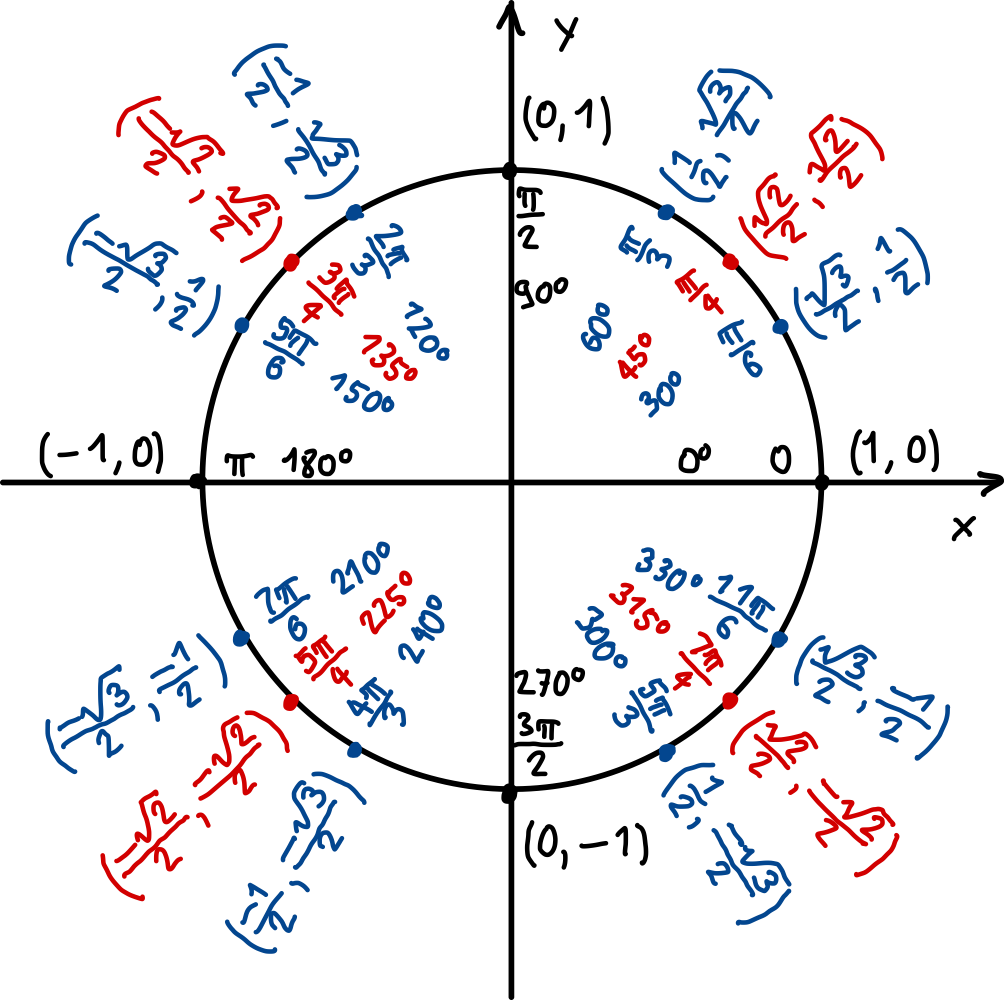
\includegraphics[width=\linewidth]{Einheitskreis.png}
\end{center}

\section{Tabellen}
\small
\subsection{Grenzwerte}
\begin{center}
  \begin{tabularx}{\linewidth}{XX}
    \toprule
    $\displaystyle \limxi \frac{1}{x} = 0$ &
    $\displaystyle \limxi 1 + \frac{1}{x} = 1$ \\
    $\displaystyle \limxi e^x = \infty$ &
    $\displaystyle \limxn e^x = 0$ \\
    $\displaystyle \limxi e^{-x} = 0$ &
    $\displaystyle \limxn e^{-x} = \infty$ \\
    $\displaystyle \limxi \frac{e^x}{x^m} = \infty$ &
    $\displaystyle \limxn xe^x = 0$ \\
    $\displaystyle \limxi \ln(x) = \infty$ &
    $\displaystyle \limxo \ln(x) = -\infty$ \\
    $\displaystyle \limxi (1+x)^{\frac{1}{x}} = 1$ &
    $\displaystyle \limxo (1+x)^{\frac{1}{x}} = e$ \\
    $\displaystyle \limxi (1+\frac{1}{x})^b = 1$ &
    $\displaystyle \limxi n^{\frac{1}{n}} = 1$ \\
    $\displaystyle \lim_{x\to\pm\infty} (1 + \frac{1}{x})^x = e$ &
    $\displaystyle \limxi (1-\frac{1}{x})^x = \frac{1}{e}$ \\
    $\displaystyle \lim_{x\to\pm\infty} (1 + \frac{k}{x})^{mx} = e^{km}$ &
    $\displaystyle \limxi (\frac{x}{x+k})^x = e^{-k}$ \\
    $\displaystyle \limxo \frac{a^x -1}{x} = \ln(a), \; \forall a > 0$ &
    $\displaystyle \limxi x^a q^x = 0, \; \forall 0 \le q < 1$ \\
    $\limxo \frac{\sin x}{x} = 1$ & $\limxo \frac{\sin kx}{x} = k$\\
    $\limxo \frac{1}{\cos x} = 1$ & $\limxo \frac{\cos x -1}{x} = 0$ \\
    $\limxo \frac{\log 1 - x}{x} = -1$ & $\limxo x \log x = 0$\\
    $\limxo \frac{1 - \cos x}{x^2} = \frac{1}{2}$ & $\limxo \frac{e^x-1}{x} = 1$ \\
    $\limxo \frac{x}{\arctan x} = 1$ & $\limxi \arctan x = \frac{\pi}{2}$ \\
    $\limxo \frac{e^{ax}-1}{x} = a$ & $\limxo \frac{\ln(x+1)}{x} = 1$ \\
    $\lim_{x\to 1} \frac{\ln(x)}{x-1} = 1$ & $\limxi \frac{\log(x)}{x^a} = 0$ \\
    $\limxi \sqrt[x]{x} = 1$ & $\limxi \frac{2x}{2^x} = 0$ \\
    \bottomrule
  \end{tabularx}
\end{center}

\subsection{Ableitungen}
\begin{center}
  % the c>{\centering\arraybackslash}X is a workaround to have a column fill up all space and still be centered
  \begin{tabularx}{\linewidth}{c>{\centering\arraybackslash}Xc}
  \toprule
  $\displaystyle \mathbf{F(x)}$ &
  $\displaystyle \mathbf{f(x)}$ &
  $\displaystyle \mathbf{f'(x)}$ \\
  \midrule
  $\displaystyle \frac{x^{-a+1}}{-a+1}$ &
  $\displaystyle \frac{1}{x^a}$ &
  $\displaystyle \frac{a}{x^{a+1}}$ \\
  $\displaystyle \frac{x^{a+1}}{a+1}$ &
  $\displaystyle x^a \ (a \ne 1)$ &
  $\displaystyle a \cdot x^{a-1}$ \\
  $\displaystyle \frac{1}{k \ln(a)}a^{kx}$ &
  $\displaystyle a^{kx}$ &
  $\displaystyle ka^{kx} \ln(a)$ \\
  $\displaystyle \ln |x|$ &
  $\displaystyle \frac{1}{x}$ &
  $\displaystyle -\frac{1}{x^2}$ \\
  $\displaystyle \frac{2}{3}x^{3/2}$ &
  $\displaystyle \sqrt{x}$ &
  $\displaystyle \frac{1}{2\sqrt{x}}$\\
  $\displaystyle -\cos(x)$ &
  $\displaystyle \sin(x)$ &
  $\displaystyle \cos(x)$ \\
  $\displaystyle \sin(x)$ &
  $\displaystyle \cos(x)$ &
  $\displaystyle -\sin(x)$ \\
  $\displaystyle \frac{1}{2}(x-\frac{1}{2}\sin(2x))$ &
  $\displaystyle \sin^2(x)$ &
  $\displaystyle 2 \sin(x)\cos(x)$ \\
  $\displaystyle \frac{1}{2}(x + \frac{1}{2}\sin(2x))$ &
  $\displaystyle \cos^2(x)$ &
  $\displaystyle -2\sin(x)\cos(x)$ \\
  \multirow{2}*{$\displaystyle -\ln|\cos(x)|$} &
  \multirow{2}*{$\displaystyle \tan(x)$} &
  $\displaystyle \frac{1}{\cos^2(x)}$  \\
  &
  &
  $\displaystyle 1 + \tan^2(x)$ \\
  $\displaystyle \cosh(x)$ &
  $\displaystyle \sinh(x)$ &
  $\displaystyle \cosh(x)$ \\
  $\displaystyle \log(\cosh(x))$ &
  $\displaystyle \tanh(x)$ &
  $\displaystyle \frac{1}{\cosh^2(x)}$ \\
  $\displaystyle \ln | \sin(x)|$ &
  $\displaystyle \cot(x)$ &
  $\displaystyle -\frac{1}{\sin^2(x)}$ \\
  $\displaystyle \frac{1}{c} \cdot e^{cx}$ &
  $\displaystyle e^{cx}$ &
  $\displaystyle c \cdot e^{cx}$ \\
  $\displaystyle x(\ln |x| - 1)$ &
  $\displaystyle \ln |x|$ &
  $\displaystyle \frac{1}{x}$ \\
  $\displaystyle \frac{1}{2}(\ln(x))^2$ &
  $\displaystyle \frac{\ln(x)}{x}$ &
  $\displaystyle \frac{1 - \ln(x)}{x^2}$ \\
  $\displaystyle \frac{x}{\ln(a)} (\ln|x| -1)$ &
  $\displaystyle \log_a |x|$ &
  $\displaystyle \frac{1}{\ln(a)x}$ \\
  \bottomrule
  \end{tabularx}
\end{center}

\subsection{Weitere Ableitungen}
\begin{center}
  \begin{tabularx}{\linewidth}{>{\centering\arraybackslash}X>{\centering\arraybackslash}X}
  \toprule
  $\displaystyle \mathbf{F(x)}$ &
  $\displaystyle \mathbf{f(x)}$ \\
  \midrule
  $\displaystyle \arcsin(x)$ &
  $\displaystyle \frac{1}{\sqrt{1 - x^2}}$ \\
  $\displaystyle \arccos(x)$ &
  $\displaystyle \frac{-1}{\sqrt{1 - x^2}}$ \\
  $\displaystyle \arctan(x)$ &
  $\displaystyle \frac{1}{1 + x^2}$ \\ 
  $\displaystyle x^x \ (x > 0)$ &
  $\displaystyle x^x \cdot (1 + \ln x)$ \\
  \bottomrule
  \end{tabularx}
\end{center}

\subsection{Integrale}
\begin{center}
\begin{tabularx}{\linewidth}{>{\centering\arraybackslash}X>{\centering\arraybackslash}X}
 \toprule
 $\displaystyle \mathbf{f(x)}$ &
 $\displaystyle \mathbf{F(x)}$ \\
 \midrule
 $\displaystyle \int f'(x) f(x) \dx$ &
 $\displaystyle \frac{1}{2}(f(x))^2$ \\
 $\displaystyle \int \frac{f'(x)}{f(x)} \dx$ &
 $\displaystyle \ln|f(x)|$ \\
 $\displaystyle \int_{-\infty}^\infty e^{-x^2} \dx$ &
 $\displaystyle \sqrt{\pi}$ \\
 $\displaystyle \int (ax+b)^n \dx$ &
 $\displaystyle \frac{1}{a(n+1)}(ax+b)^{n+1}$ \\
 $\displaystyle \int x(ax+b)^n \dx$ &
 $\displaystyle \frac{(ax+b)^{n+2}}{(n+2)a^2} - \frac{b(ax+b)^{n+1}}{(n+1)a^2}$ \\
 $\displaystyle \int (ax^p+b)^n x^{p-1} \dx$ &
 $\displaystyle \frac{(ax^p+b)^{n+1}}{ap(n+1)}$ \\
 $\displaystyle \int (ax^p + b)^{-1} x^{p-1} \dx$ &
 $\displaystyle \frac{1}{ap} \ln |ax^p + b|$ \\
 $\displaystyle \int \frac{ax+b}{cx+d} \dx$ &
 $\displaystyle \frac{ax}{c} - \frac{ad-bc}{c^2} \ln |cx +d|$ \\
 $\displaystyle \int \frac{1}{x^2+a^2} \dx$ &
 $\displaystyle \frac{1}{a} \arctan \frac{x}{a}$ \\
 $\displaystyle \int \frac{1}{x^2 - a^2} \dx$ &
 $\displaystyle \frac{1}{2a} \ln\left| \frac{x-a}{x+a} \right|$ \\
 $\displaystyle \int \sqrt{a^2+x^2} \dx $ &
 $\displaystyle \frac{x}{2}f(x) + \frac{a^2}{2}\ln(x+f(x))$ \\
 \bottomrule
\end{tabularx}
\end{center}

\section{Quellen}
Ein Grossteil des Cheatsheets wurde stark vom Cheatsheet von Ruben Schenk (\href{https://rwgs.ch}{https://rwgs.ch}) und vom PVW Skript (\href{https://vis.ethz.ch/de/services/pvw-scripts/}{https://vis.ethz.ch/de/services/pvw-scripts/}) inspiriert. Ausserdem stammen Teile der Tabellen aus dem Buch ``Formeln, Tabellen und Konzepte''. Schliesslich sind die Definitionen meistens dem Skript ``Analysis 1'' von Marc Burger entnommen.


\end{document}